\documentclass[12pt,oneside,a4paper,english]{article}
\usepackage[T1]{fontenc}
\usepackage[latin2]{inputenc}
\usepackage[margin=2.25cm,headheight=26pt,includeheadfoot]{geometry}
\usepackage[english]{babel}
\usepackage{listings}
\usepackage{color}
\usepackage{titlesec}
\usepackage{titling}
\usepackage[framed, numbered]{matlab-prettifier}
\usepackage{changepage}
\usepackage{amsmath}
\usepackage{hyperref}
\usepackage{enumitem}
\usepackage{graphicx}
\usepackage{fancyhdr}
\usepackage{lastpage}
\usepackage{caption}
\usepackage{tocloft}
\usepackage{setspace}
\usepackage{multirow}
\usepackage{titling}
\usepackage{float}
\usepackage{comment}
\usepackage{booktabs}
\usepackage{indentfirst}
\usepackage{lscape}
\usepackage{booktabs,caption}
\usepackage[flushleft]{threeparttable}
\usepackage[english]{nomencl}
\usepackage{xcolor}
\usepackage{lipsum}
\usepackage{pythonhighlight}

% --- set footer and header ---
\pagestyle{fancy}
\fancyhf{}

\setlength{\parindent}{2em}
\title{RF-based positioning for UAVs} % to reference as \title, dont use \maketitle
\makeatletter\let\Title\@title\makeatother

\lstset{language=Matlab,
style=Matlab-editor,
basicstyle=\normalsize\mlttfamily,
numbers=left,
numberstyle={\scriptsize\color{black}},			% size of the numbers
numbersep=0.5cm											
}

\newlist{steps}{enumerate}{1}
\setlist[steps, 1]{leftmargin=1.5cm,label = Step \arabic*:}
\renewcommand{\headrulewidth}{1pt}
\renewcommand{\footrulewidth}{1pt}

%\lhead{\Title}
\rhead{\nouppercase{\rightmark}}
\lhead{\Title}
\rfoot{
\includegraphics[height=1.25cm]{root/logo.pdf}} % right header logo
\setlength\headheight{16pt}
\setlength{\footskip}{50pt}
\lhead{\Title} %rightH title
\cfoot{\thepage}

% --- End of page settings ---

\begin{document}
\pagenumbering{roman}

\begin{titlepage}
\begin{center}
\vspace{2cm}
%\textsc{ Danmarks Tekniske Universitet}\\[1.5cm]

\includegraphics[width=0.4\textwidth]{root/dtu.png}~\\[1cm]
\vspace{2cm}

\vspace{2cm}

% Title
\hrule
\vspace{.5cm}
{ \huge \bfseries RF-based positioning for\\ }
\vspace{.1cm}
{ \huge \bfseries Unmanned Autonomous Vehicles}
\vspace{.5cm}

\hrule
\vspace{1.5cm}

\textsc{\textbf{Author}}\\
\vspace{.5cm}
\centering

Ernestas Simutis - s212571\\
\vspace{.5cm}

\textsc{\textbf{Supervisors}}\\
\vspace{.5cm}
\centering

Matteo Fumagalli\\
Jeppe Heini Mikkelsen\\
Peter Iwer Hoedt Karstensen\\

\vspace*{\fill}

\centering \today
\end{center}
\end{titlepage}



\newpage
\doublespacing
\renewcommand{\baselinestretch}{1}\normalsize
\tableofcontents
\renewcommand{\baselinestretch}{1}\normalsize
\thispagestyle{fancy} % force page style

\newpage
\pagenumbering{arabic}
\fancyfoot[C]{Page \thepage\ of \pageref{EndOfText}}

\section{Project Goals} \label{ch1}
\begin{itemize}
    \item Investigate different RF technologies for positioning and evaluate their pros and cons, e.g. WiFi, UWB, BLE, etc.
    \item Implement an RF based range measurement method
    \item Compare range measurement using RSSI (Received Signal Strength Indication) and RTT (Round Trip Time)
    \item Implement a Bayesian filter for positioning using aforementioned range measurement(s)
\end{itemize}

\newpage

\section{RF-based positioning} \label{ch2}

RF (radio frequency) based positioning problem is concerned with inferring agent/robot position in space from distance measurements to a number of known static or dynamic beacons/landmarks. For instance, in three dimensional case position can be computed by having at least three distance measurements. Technique for doing this is called multilateration.

The chapter is divided in a following way: first describing general methods of measuring distance between two RF devices/antennas, secondly investigating existing protocols making measurements and lastly selecting an algorithm to iteratively compute and track position of a robot over time.

% TODO: put it in a better way : )
Requirements for application:
\begin{itemize}
    \item Ranging max distance - at least 100 meters.
\end{itemize}

\subsection{Range measurement methods}

Literature points out two main methods for making distance measurements over RF antennas: RSSI (Received Signal Strength Indication) and time based methods.
% TODO: AoA?

\subsubsection{RSSI}

As the name suggests the received signal strength hints at the power of incoming radio signal. There is non-linear corelation between RSSI and distance between two antennas \cite{rssi-curves}:
$$
R S S I=-10 n \log _{10}(d)+C
$$
thus it is possible, for instance, to fit a curve on a measured experimental values like shown in \cite{rssi-curves}. However, the main disadvantage that for commercial protocols the quantity over distance curve flattens out at certain distance and further it's impossible to tell the a difference between different measurements. The effect can be seen in Figure \ref{fig:rssi-curves}. Due to this limitation the method is not suitable according to application requirements thus later comparison of available RF technologies for positioning will focus mainly on time based methods.
\begin{figure}
    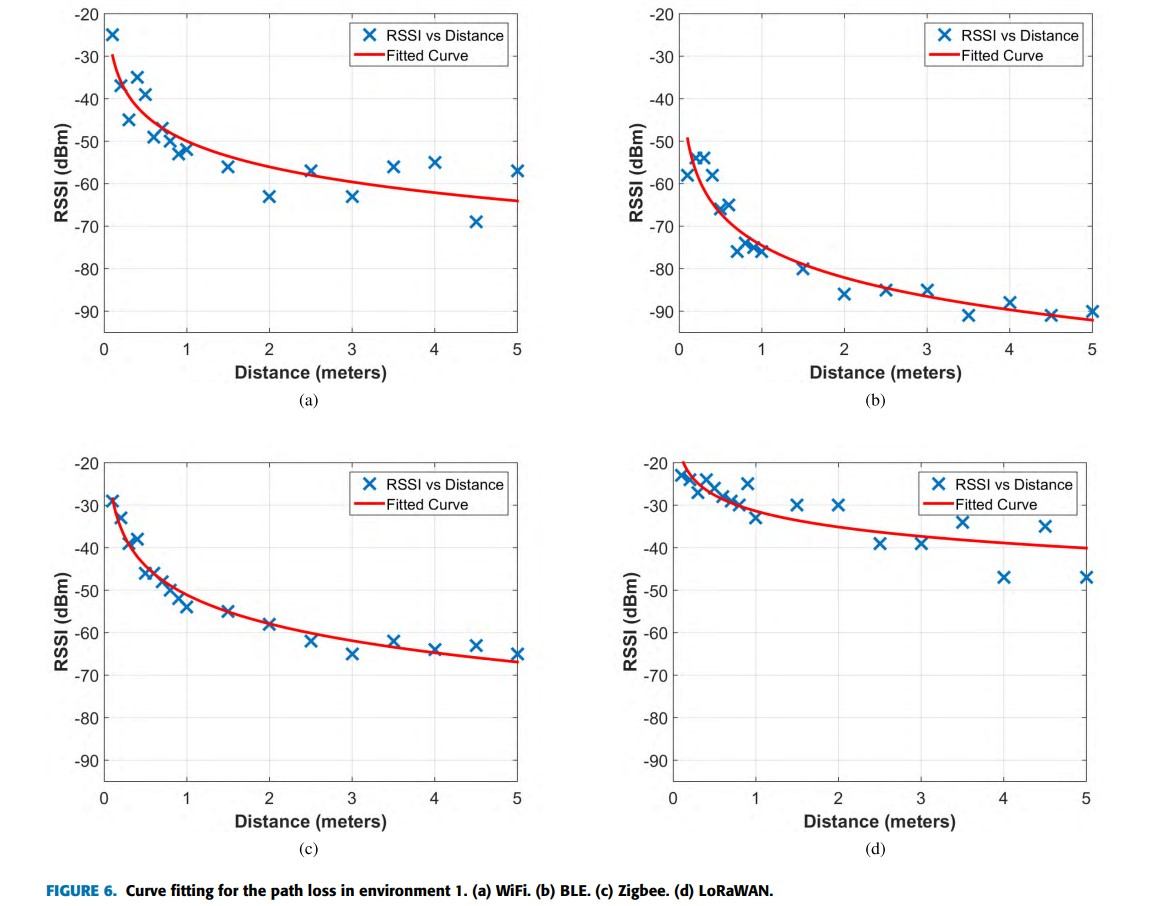
\includegraphics[width=\linewidth]{figures/RSSICurves.jpg}
    \caption{Various protocol RSSI over distance curves \cite{rssi-curves}.}
    \label{fig:rssi-curves}
\end{figure}
  
\subsubsection{Time based}

These methods are based on measuring radio wave propagation time between (or ToF - \emph{Time of Flight}) antennas/devices and calculating the distance by knowing light speed i.e. $d=ct$, where $c=10e-8$ m/s. One obvious drawback here is that two clock must be synchronized if to infer the distance by ToA (\emph{Time of Arrival}). However, this can be avoided by doing a round trip (in literature referred as TDoA - \emph{Time Difference of Arrival}) and relying solely on one clock. The scheme is illustrated in \ref{fig:RTT} where $T_{prop}$ is propagation time in which we are interested in for ranging applications. The value can be computed by $T_{prop} = \frac{1}{2}(T_{round} - T_{reply})$. Also, Figure \ref{fig:RTT} correctly indicates the scale of $T_{round}$ and $T_{prop}$. Important thing to notice here, if the distances we're measuring are in order of meters, $T_{prop} = d/c$ evaluates to nanosecond scale while for response computer might have to execute hundreds of instructions taking up way more time than the time we're interested in. Thus it's of most importance to know how much time computation takes in the responding device. When selecting/designing a system to use RTT for positioning, responding device must have very fine granularity control of computing resources. If one would try to make these computations on OS (Operating system) level, the time jitter introduced by OS scheduling system would be so large that propagation time would vanish in the error of $T_{reply}$ measurement.
\begin{figure}[H]
    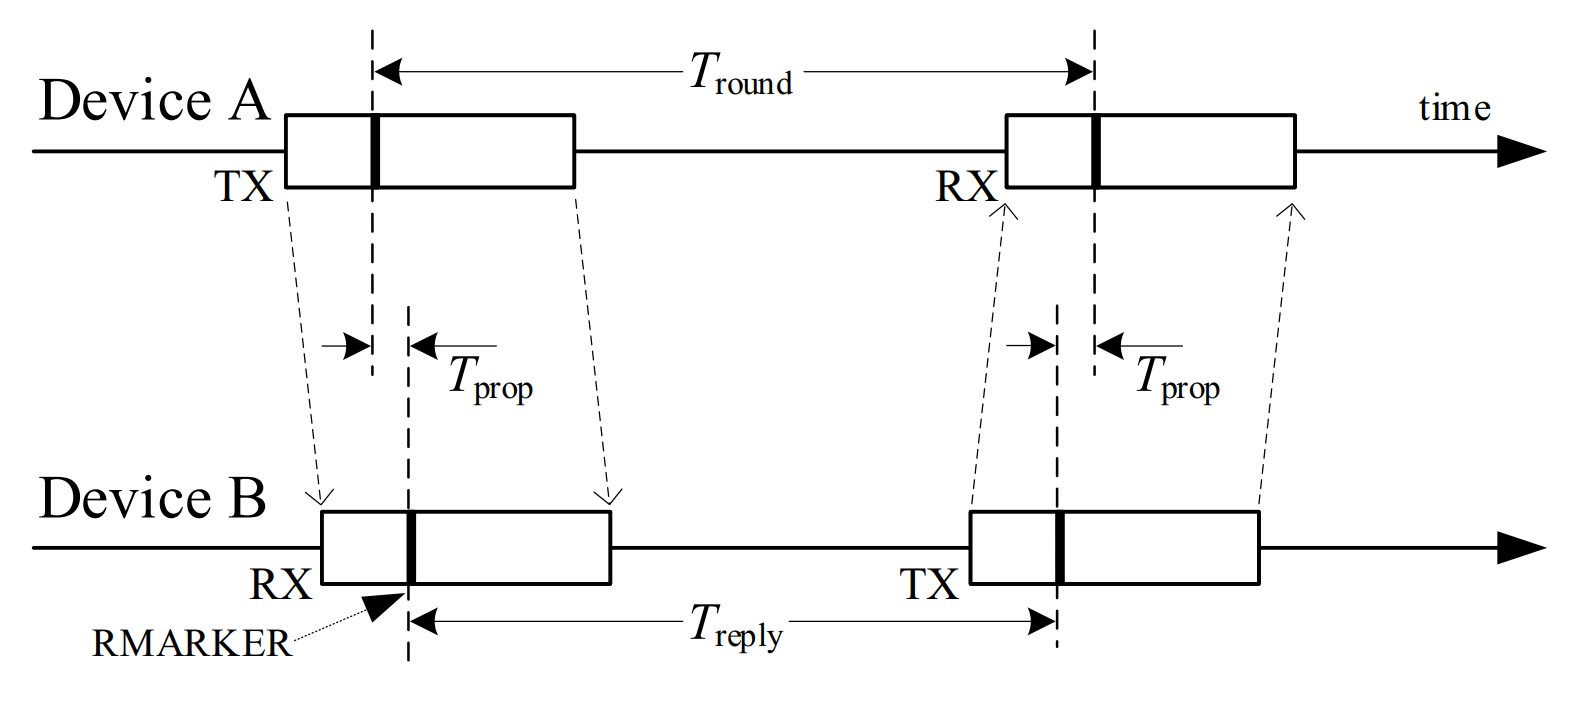
\includegraphics[width=\linewidth]{figures/RTT.jpg}
    \caption{Round trip time \cite{9179124}.}
    \label{fig:RTT}
\end{figure}
  
\subsection{RF positioning}

There are many existing protocols/technologies to exchange data between devices over the air i.e. by transmitting it over electromagnetic waves. In this chapterF, a few of most popular ones will be reviewed in terms of how suitable each of them is for positioning applications. Namely, paper investigates WiFi, UWB (Ultra Wide Band) and BLE (Bluetooth Low Energy) protocols.

\subsubsection{WiFi}

FTM RTT: RTT could be obtained by FTM protocol but is difficult to obtain bc hardware support is very limited. Even then requires quite a bit of effort to install required driver, firmware, kernel version. The distance measurement is not that precise. Best case scenario gives 1-2m accuracy which is nice but more crude estimation would also work.
% https://www.banshee-navigation.eu/blog/posts/what_is_wi-fi_rtt
% https://www.winlab.rutgers.edu/~gruteser/projects/ftm/Setups.htm

Positioning base on WiFi signal strength is way easier. Basically could be implemented with any WiFi card without spending additional time on setup. Accuracy is worse ~10m. But meets the requirements and prob is worth trying first before going to alternatives. Turns out that the distance to signal curve flattens out at around 20m and cannot measure distances beyond that...
% TODO:

So wifi frequency is max 80MHz which in time based methods alone results in max theoretical distance resolution of 3.5m of time based methods.

% TODO:
% Measuring Round Trip Times to Determine the Distance Between WLAN Nodes 803 pdf page; data collection & processing https://link.springer.com/content/pdf/10.1007/b136094.pdf
% The resolution of these hardware time stamps, which are implemented in most current WLAN products, is 1 μs corresponding to 300 m. :D and they  don't say how they get those hardware timestamps either, mistery still.

% TODO:
% why some papers say that distance resolution is dependant on bandwidth? even though the wifi freq is 2.4 of 5 GHz. How come the distance resolution calculation only takes in bandwidth for example 20MHz or 40MHz???
% https://github.com/domienschepers/wifi-ftm

\subsubsection{BLE}

Easily available but no support for precision time stamping...

\subsubsection{UWB}

How does UWB solve time stamping? THis is very well defined in the official standard 802154z-2020, read the pdf and do a summary.
% https://www.mouser.dk/ProductDetail/Qorvo/DWM3000EVB?qs=iLbezkQI%252BsgO%252Bhh8kPU5Xg%3D%3D
% https://www.mouser.dk/new/qorvo/qorvo-dws3000evb-arduino-shield/
% https://github.com/Makerfabs/Makerfabs-ESP32-UWB
% https://arxiv.org/pdf/2202.02190.pdf check this out too, An Overview of UWB Standards

\subsection{Position from distance measurement}

However, solution (from 3 beacons) is not unique and adding fourth one allows to come up with a distinctive robot position easier.

\newpage

\section{Positioning} \label{ch3}
Chapter covers application and implementation of EKF (Extended Kalman Filter) for estimation of 3D position in space and writing a simulation to validate the filter implementation.

\subsection{EKF}

Due to sensor measurement noise state estimator is necessary. Thus Kalman filter will be implemented and deployed to track agents position assuming noisy observations of distance. Before going into details it's important to think about state evolution and observation models because Kalman filter assumes both to be linear. During project constant velocity model will be used, described by:
$$
    \left[\begin{array}{c}
            x_{k+1}       \\
            y_{k+1}       \\
            z_{k+1}       \\
            \dot{x}_{k+1} \\
            \dot{y}_{k+1} \\
            \dot{z}_{k+1}
        \end{array}\right]=\left[\begin{array}{cccccc}
            1 & 0 & 0 & \Delta t & 0        & 0        \\
            0 & 1 & 0 & 0        & \Delta t & 0        \\
            0 & 0 & 1 & 0        & 0        & \Delta t \\
            0 & 0 & 0 & 1        & 0        & 0        \\
            0 & 0 & 0 & 0        & 1        & 0        \\
            0 & 0 & 0 & 0        & 0        & 1
        \end{array}\right]\left[\begin{array}{c}
            x_{k}       \\
            y_{k}       \\
            z_{k}       \\
            \dot{x}_{k} \\
            \dot{y}_{k} \\
            \dot{z}_{k}
        \end{array}\right]
$$
or
$$
    \boldsymbol{x}_{k+1} = \boldsymbol{F} \boldsymbol{x}_k
$$
which is linear by itself. If it were a system like drone model would be non-linear, more complex and include actuation signal in state transition. Yet the project is aiming at investigating plausibility of localization with UWB antennas rather and experiment will be done by carrying agent device while walking. This cannot be modeled and can be treated as  a black box constant velocity model.
% https://arxiv.org/pdf/2005.00844.pdf (Derivation of a Constant Velocity Motion Model for Visual Tracking) Could be useful ?

However, Euclidean distance measurement model (from beacon to agent) has non-linearity due to the \emph{norm}:
$$
    \Vert\boldsymbol{x}-\boldsymbol{b}\Vert_2 = \sqrt{{\left(\mathrm{b_x}-x\right)}^2+{\left(\mathrm{b_y}-y\right)}^2+{\left(\mathrm{b_z}-z\right)}^2}
$$
where $\boldsymbol{x} = (x,y,z)$ is vector representing agents position and $\boldsymbol{b} = (b_x,b_y,b_z)$ is position of one visible (in radio communication sense) beacon in space. This is where EKF comes into play, the method proposes to use linearized version of non-linear function by taking it's Jacobian and assuming that linearized model representation around a small deviation neighborhood holds true and usa that in place of the measurement matrix $\boldsymbol{H}$. This will be described later but, in short, one can take partial derivatives of the function with respect to each agent's position dimension and evaluate them at current state estimate. For instance:
$$
    \frac{\partial h(x)}{\partial x} = \frac{x-\mathrm{b_x}}{\sqrt{{\left(\mathrm{b_x}-x\right)}^2+{\left(\mathrm{b_y}-y\right)}^2+{\left(\mathrm{b_z}-z\right)}^2}}
$$

General discrete time EKF is defined as described in the following paragraphs, based on \cite{probrobotics} and \cite{welch1995introduction}. Starting with notation: $\hat{\mathbf{x}}_{k \mid k-1}$ represents the  estimate of $\mathbf{x}$ at time instance $k$ given observations up to and including at time $k-1$. \smallskip
% TODO: define all variables in EKF ?

\textbf{Prediction step} \smallskip
$$\hat{\boldsymbol{x}}_{k \mid k-1}=f\left(\hat{\boldsymbol{x}}_{k-1 \mid k-1}, \boldsymbol{u}_k\right)$$
$$\boldsymbol{P}_{k \mid k-1}=\boldsymbol{F}_k \boldsymbol{P}_{k-1 \mid k-1} \boldsymbol{F}_k^T+\boldsymbol{Q}_k$$

\textbf{Update step} \smallskip
$$\tilde{\boldsymbol{y}}_k=\boldsymbol{z}_k-h\left(\hat{\boldsymbol{x}}_{k \mid k-1}\right)$$
$$\boldsymbol{S}_k=\boldsymbol{H}_k \boldsymbol{P}_{k \mid k-1} \boldsymbol{H}_k^T+\boldsymbol{R}_k$$
$$\boldsymbol{K}_k=\boldsymbol{P}_{k \mid k-1} \boldsymbol{H}_k^T \boldsymbol{S}_k^{-1}$$
$$\hat{\boldsymbol{x}}_{k \mid k}=\hat{\boldsymbol{x}}_{k \mid k-1}+\boldsymbol{K}_k \tilde{\boldsymbol{y}}_k$$
$$\boldsymbol{P}_{k \mid k}=\left(\boldsymbol{I}-\boldsymbol{K}_k \boldsymbol{H}_k\right) \boldsymbol{P}_{k \mid k-1}$$
where state transition and measurement matrices are partial derivatives (\emph{Jacobians}) of state evolution and observation model functions. In constant velocity case $\boldsymbol{f}(\boldsymbol{x})$ is already linear so that part can be discarded.
$$
    \begin{aligned}
        \boldsymbol{F}_k & =\left.\frac{\partial f}{\partial \boldsymbol{x}}\right|_{\hat{\boldsymbol{x}}_{k-1 \mid k-1}, \boldsymbol{u}_k} \\
        \boldsymbol{H}_k & =\left.\frac{\partial h}{\partial \boldsymbol{x}}\right|_{\hat{\boldsymbol{x}}_{k \mid k-1}}
    \end{aligned}
$$

Distance measurement Jacobian can be computed in code by:

\begin{minipage}{\linewidth}
    \begin{python}
    def getH(x_op, beacons):
        H = np.zeros((len(beacons), len(x_op)))
        for i, b in enumerate(beacons):
        H[i][:3] = ((x_op[:3] - b.get_pos()) \
            / np.linalg.norm(x_op[:3] - b.get_pos())).T
        return H
    \end{python}
\end{minipage}
% doesn't stay formatted as i wish if i wrap it :'( despair
% \begin{figure}
%     \caption{Distance Jacobian $\boldsymbol{H} computation.$}
%     \label{code:distJ}
% \end{figure}
function takes in agent position at time $k-1$, beacon list and return partial derivatives of state variables with respect to each of the beacons. It's assumed that beacon number is fixed to 4.

\subsection{Simulation}

Figure \ref{fig:sim} shows a trail run in simulation. Please note that system state is includes the third dimension however for plotting purpose only first two components are shown. The setup is running EKF described in previous section on noisy measurement. Noise is provided by adding a random sample from Gaussian distribution to each distance measurement at every timestamp. Big $X$ is marking the start of a trajectory, $GT$ line is ground truth trajectory generated by applying state transition matrix at each instant of time (moving at arbitrary speeds to cover a rectangle), blue path is the predicted one and lastly the numbered dots represent beacons arbitrarily placed in space.
\begin{figure}[H]
    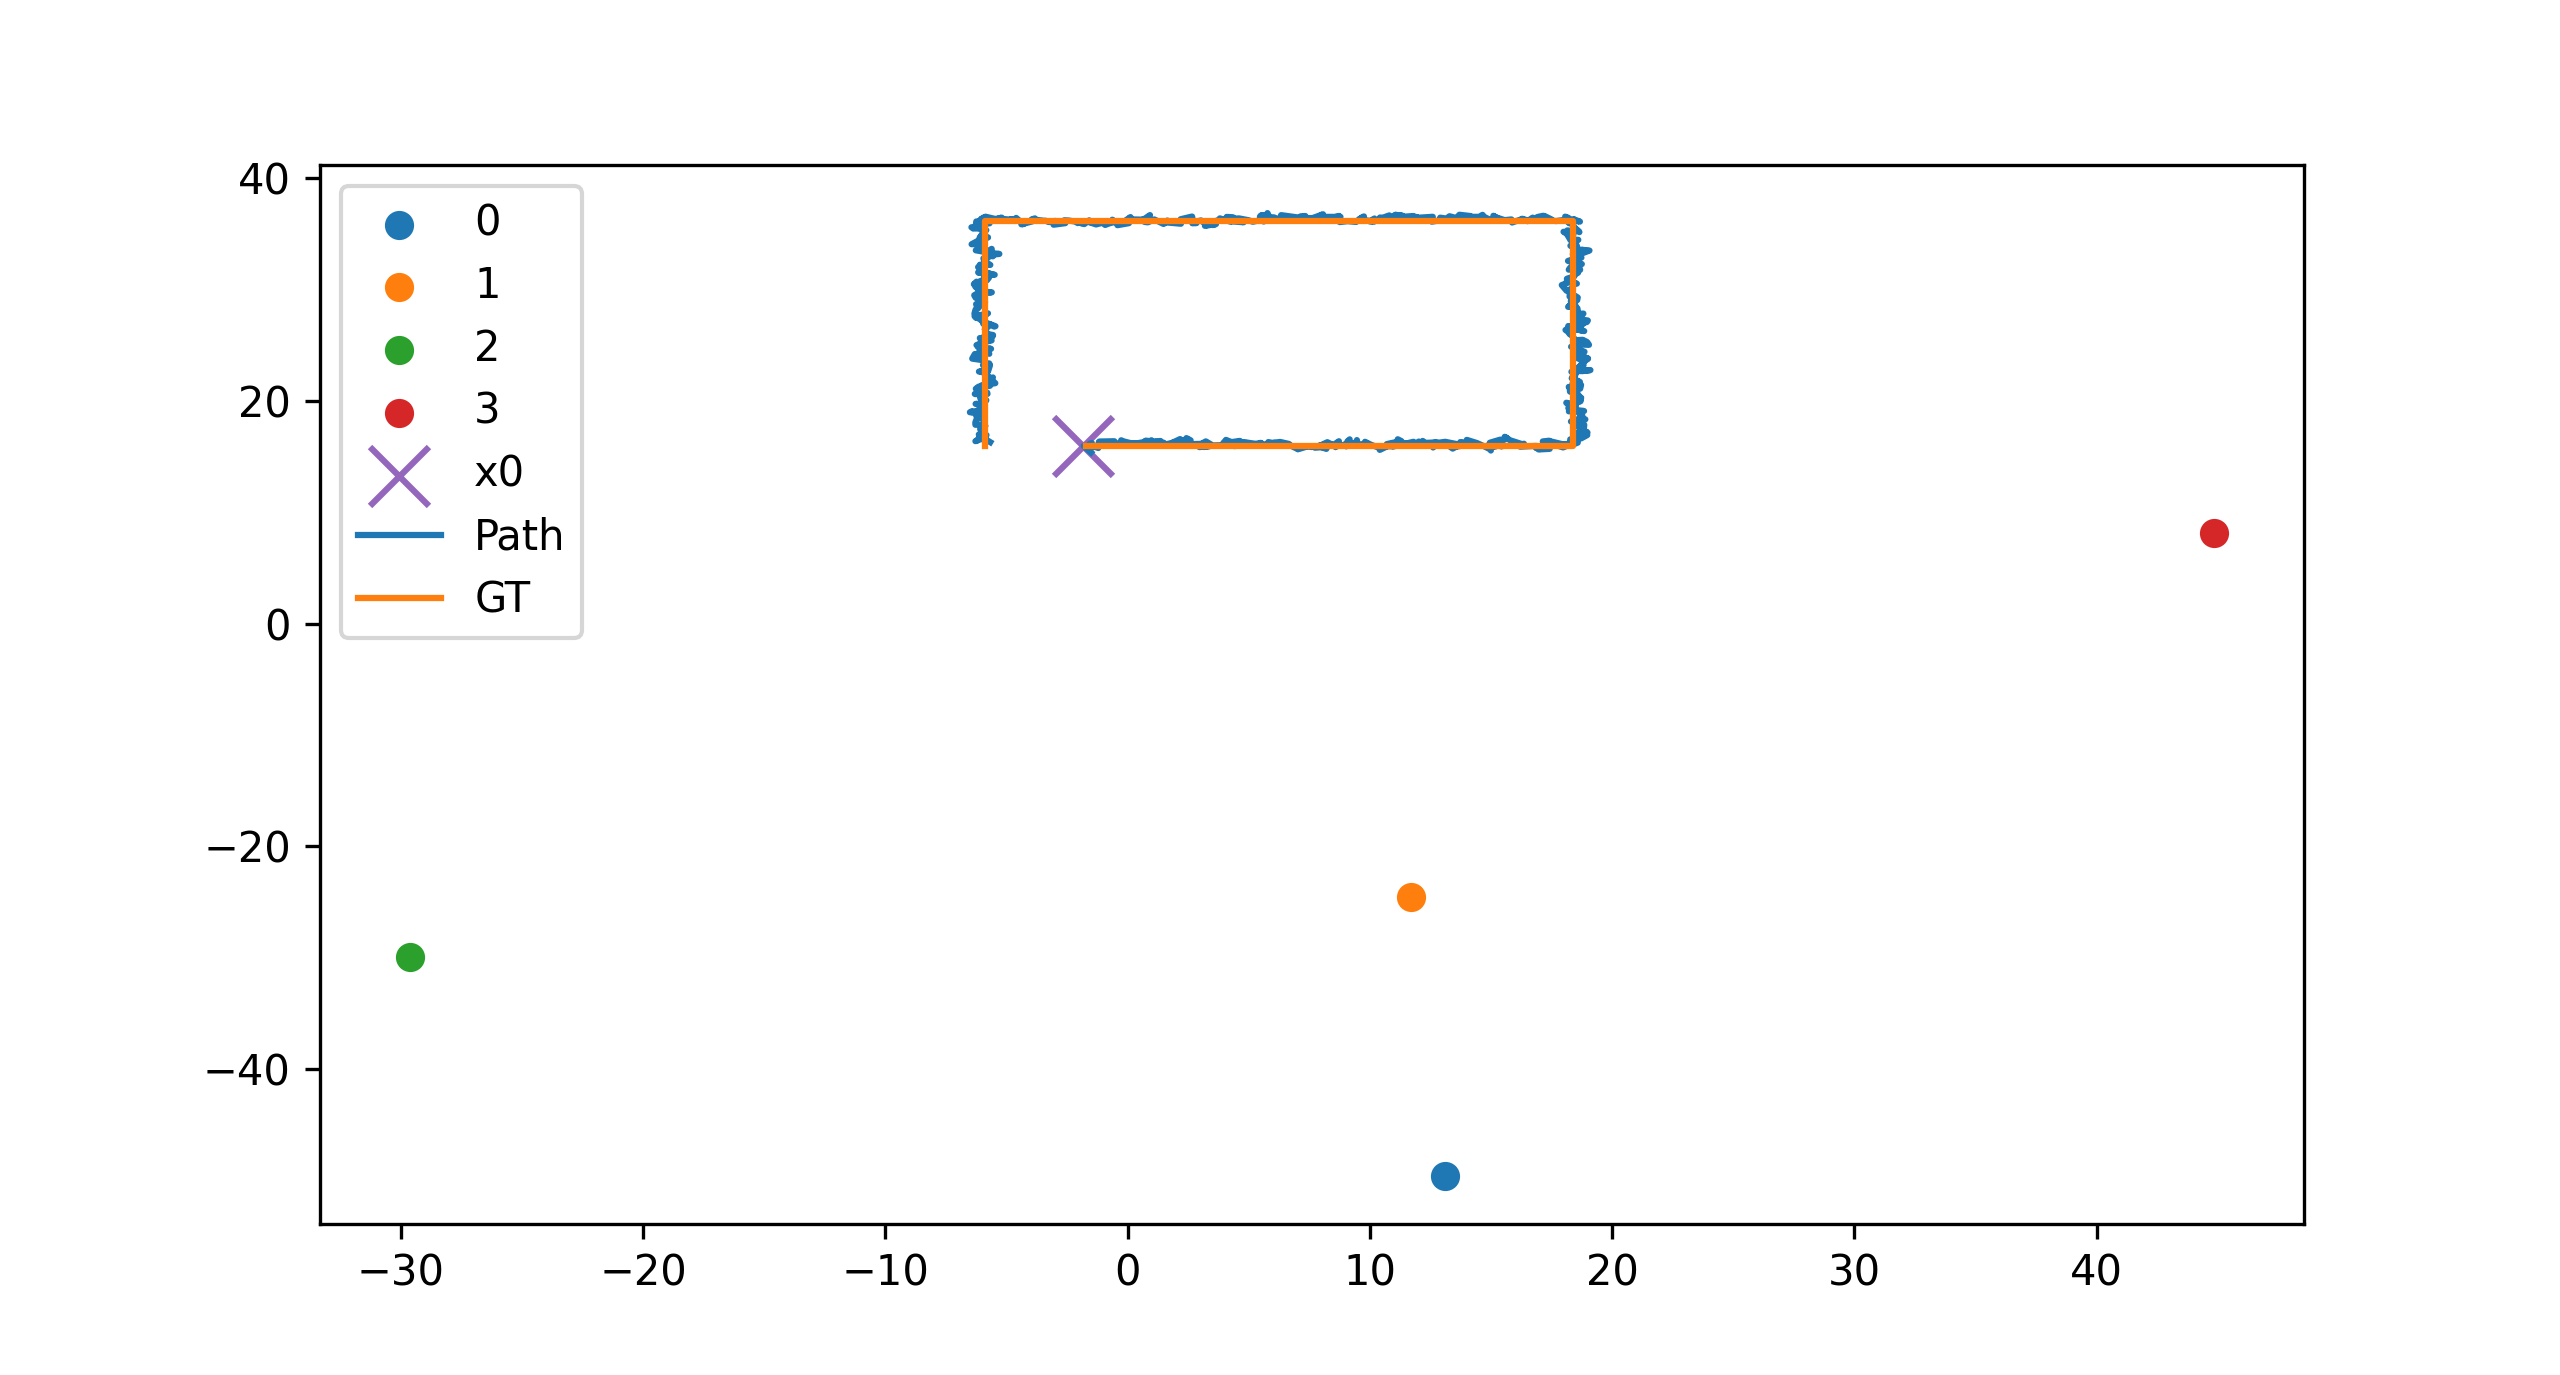
\includegraphics[width=\linewidth]{figures/sim.png}
    \caption{Simulation}
    \label{fig:sim}
\end{figure}

\newpage

\section{Experiments} \label{ch4}
Practical experiments are conducted during the course are discussed here. That includes: tuning KF (Kalman Filter) parameters (mainly evaluating covariances) by real-world experiments, testing out whole system and evaluating positioning accuracy developed in previous chapter.

\subsection{Real-world experiments}

First, it's important to address the assumption made in the simulation environment. It was assumed that sensor measurement variance is known. For filter to have good convergence properties we would like to know it up to a reasonable accuracy level when in operation. Therefore, the first experiment was conducted to measure the precision of UWB range measurements compared to a ground truth. DTU ASTA's Opticon system was used to generate ground truth labels (limited to ~10m range) and two UWB devices, one configured as a tag and another one as an anchor. During the experiment anchor was moved to different position around the track, ground truth distance calculated between devices by taking norm of two position from Opticon and corresponding measurement by the means of UWB antennas was recorded. Figure \ref{fig:distancePDF} shows the probability distributions of measured values by real-world experiments in blue and the ground truth in orange.
\begin{figure}[H]
    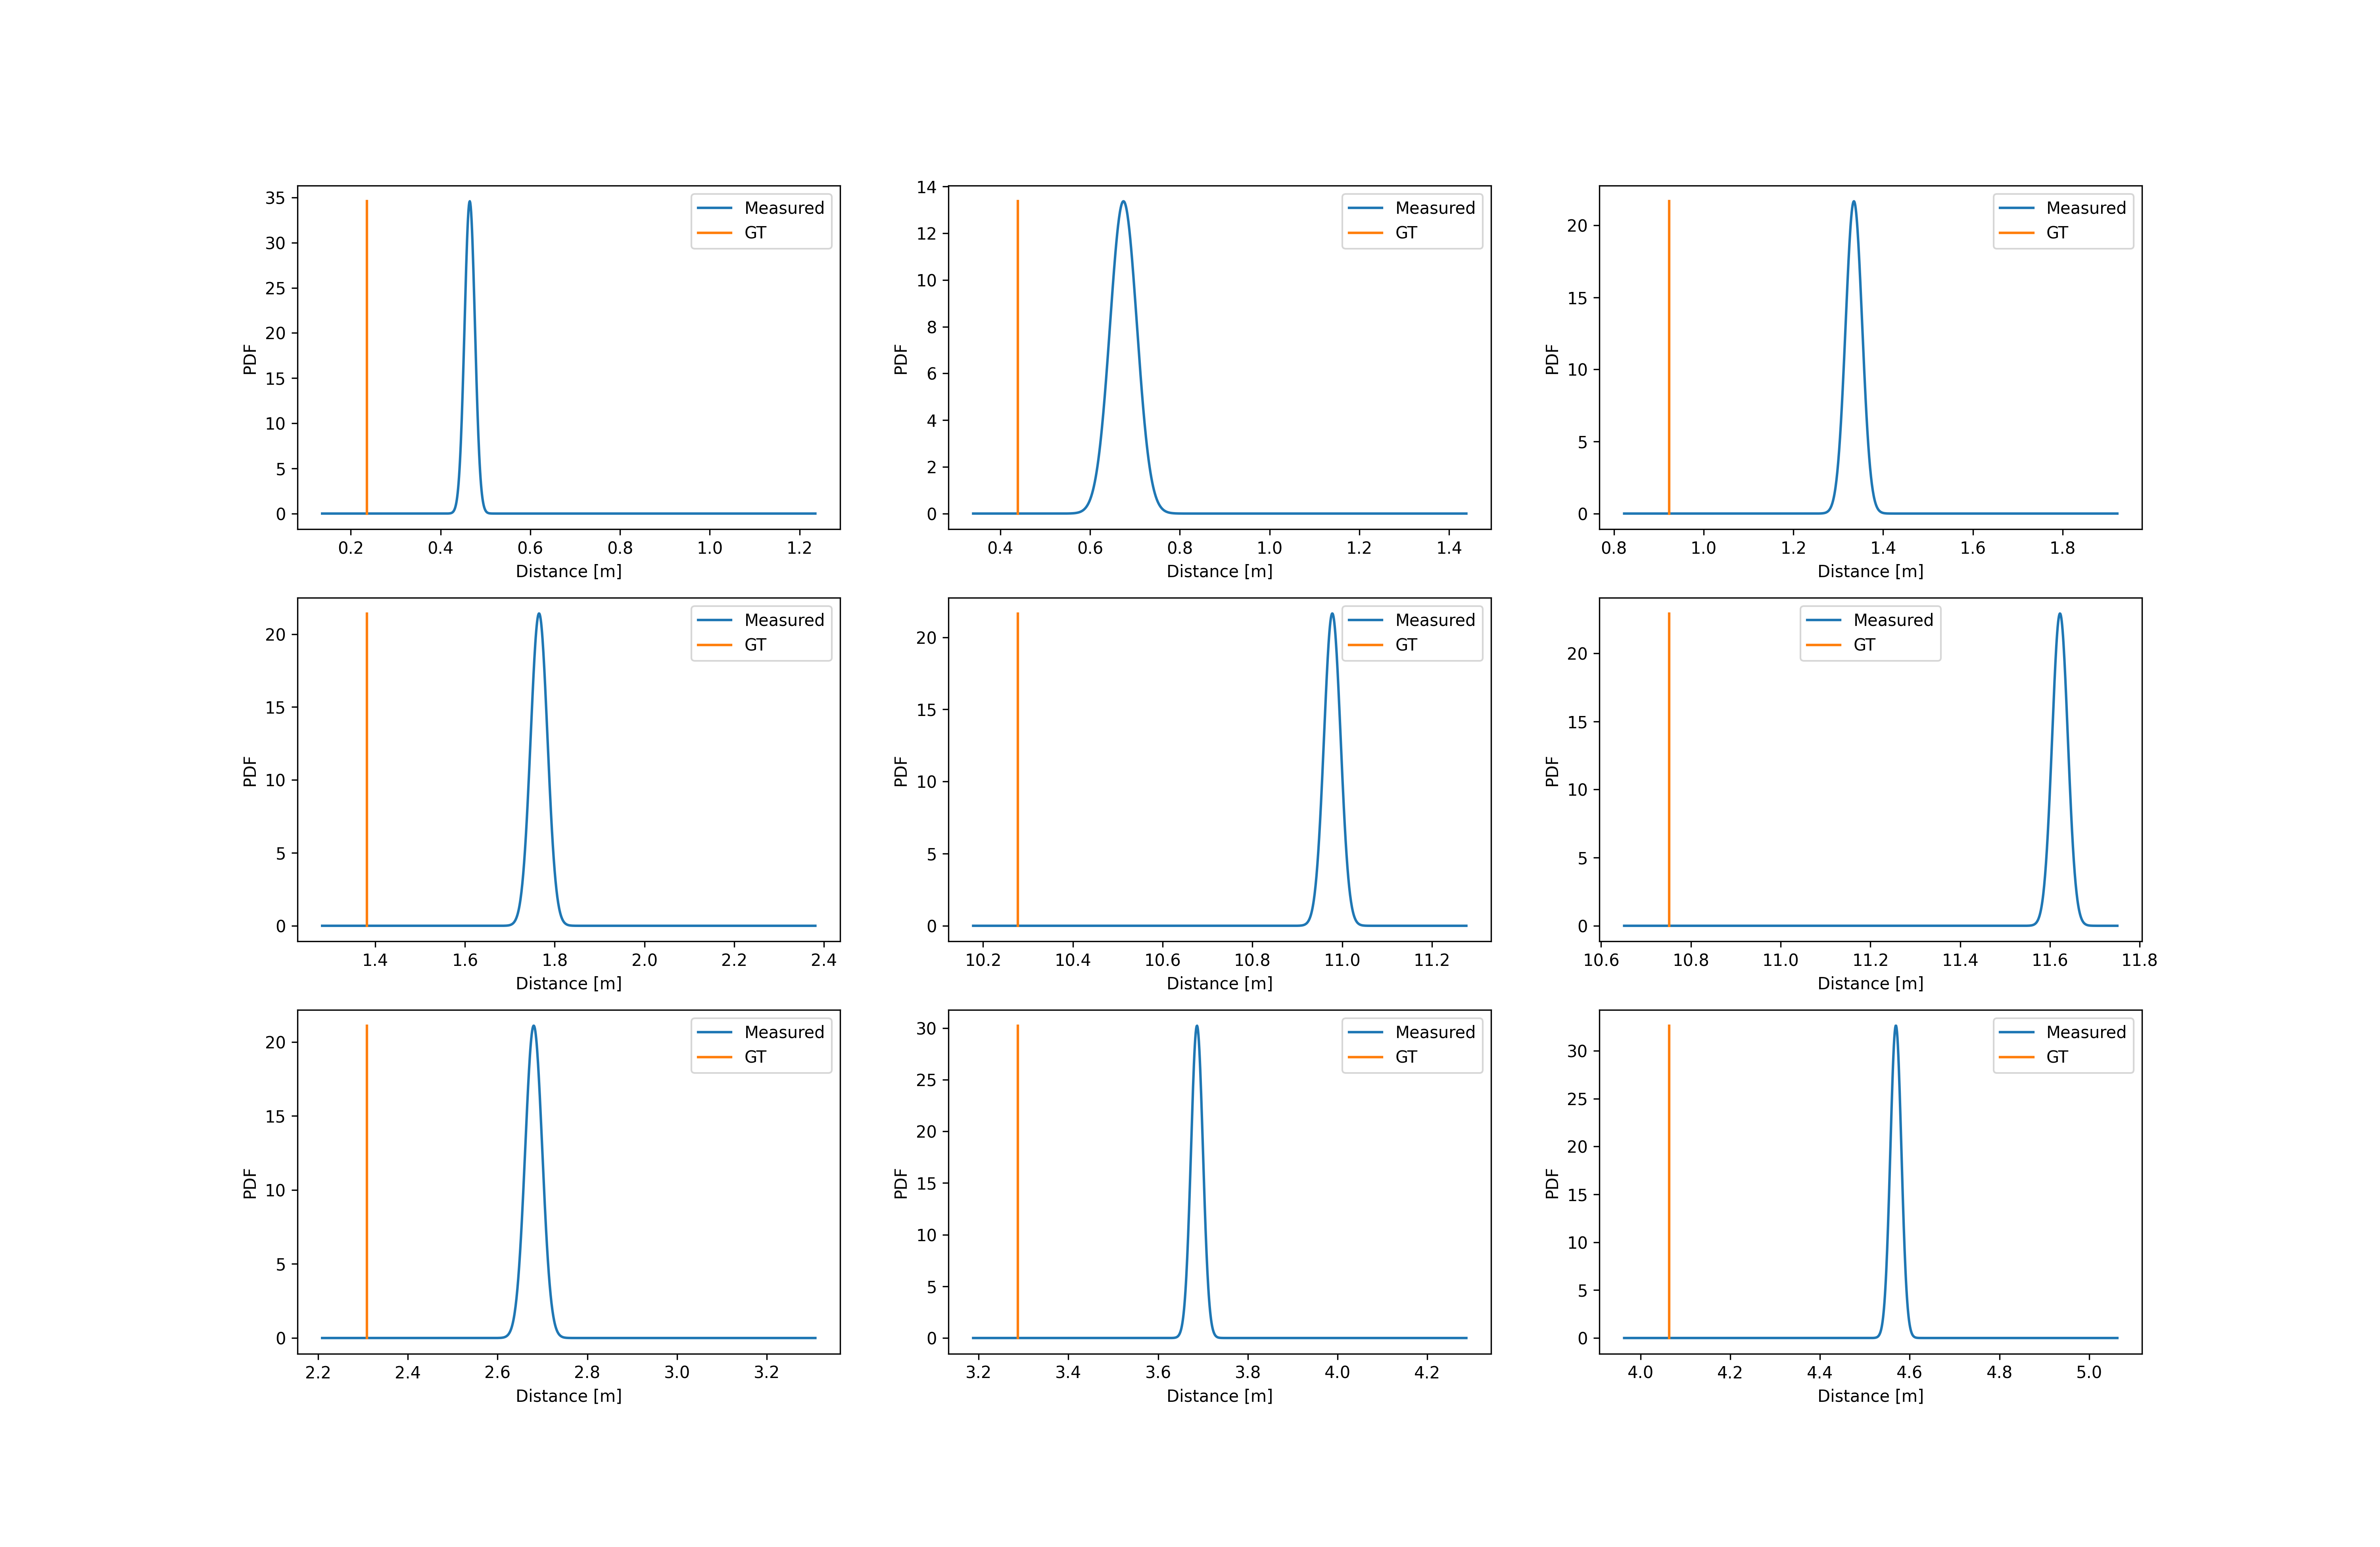
\includegraphics[width=\linewidth]{figures/distancePDF.png}
    \caption{Distance measurements PDFs.}
    \label{fig:distancePDF}
\end{figure}

Looking at the plots one noticeable thing is that mean value of measured values are shifted to the right - meaning sensor gives out bigger distance than it actually is, this could be called bias. The relationship of bias and distance is illustrated in Figure \ref{fig:distance_bias}. Additionally, it can be modeled, at least in this rang,  by a line fit, which is shown in the graph too. It approximates the bias reasonably well and will improve localization accuracy in this distance range. In a way, it's calibrating the sensor so that measurements have the same mean value as ground truths.
\begin{figure}[H]
    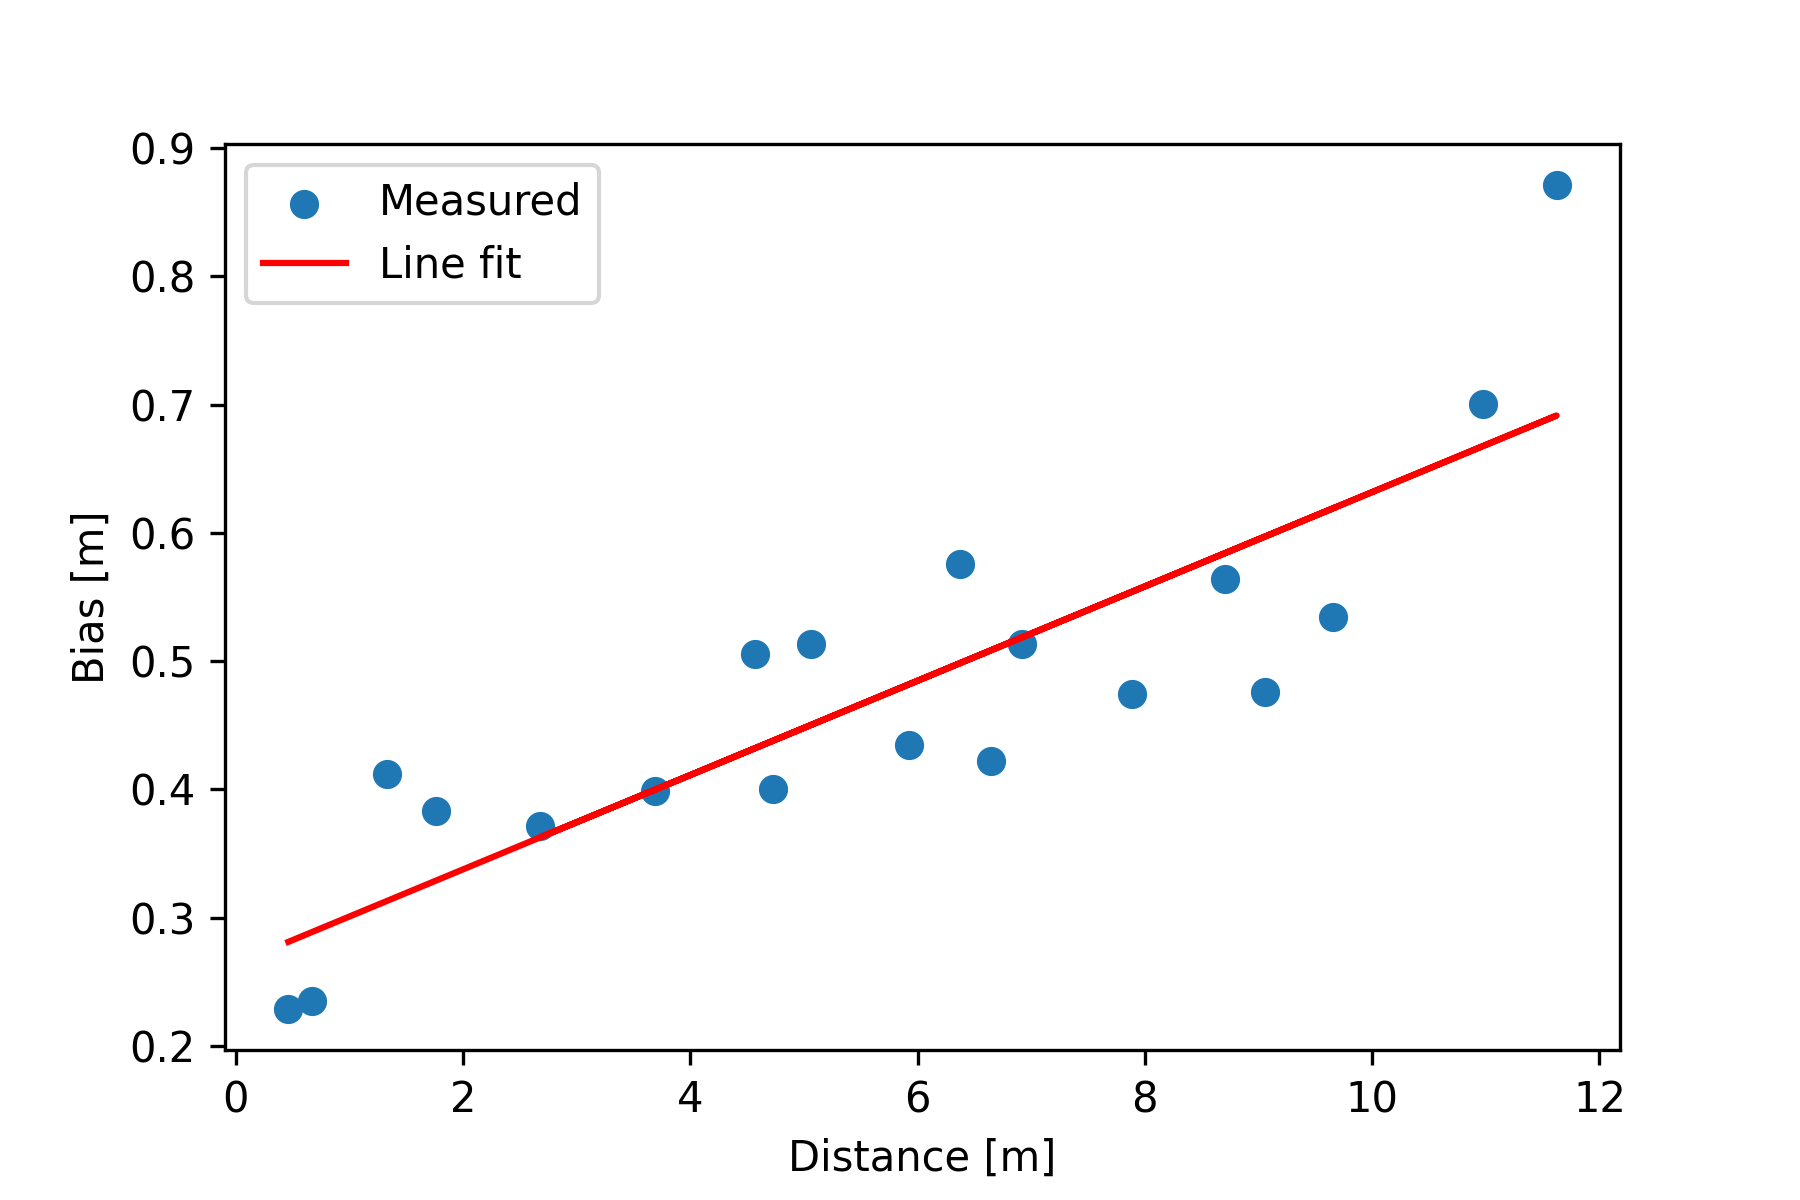
\includegraphics[width=\linewidth]{figures/distance_bias.png}
    \caption{Measurement bias over distance.}
    \label{fig:distance_bias}
\end{figure}

Next, let's look at the variance and distance relation. The question to ask here if they are dependant on each other or we can use single constant values for all range measurements. Figure \ref{fig:distance_var} shows them on single plot, plus a line fit on the data (which is, of course, bad representation of data because of one outlier). It's clearly seen that variance is very low and of almost same magnitude through out the data points. Thus, we can conclude that under tested conditions constant variance value can be used in EKF. For instance, an average value of all these variance points.
\begin{figure}[H]
    \centering
    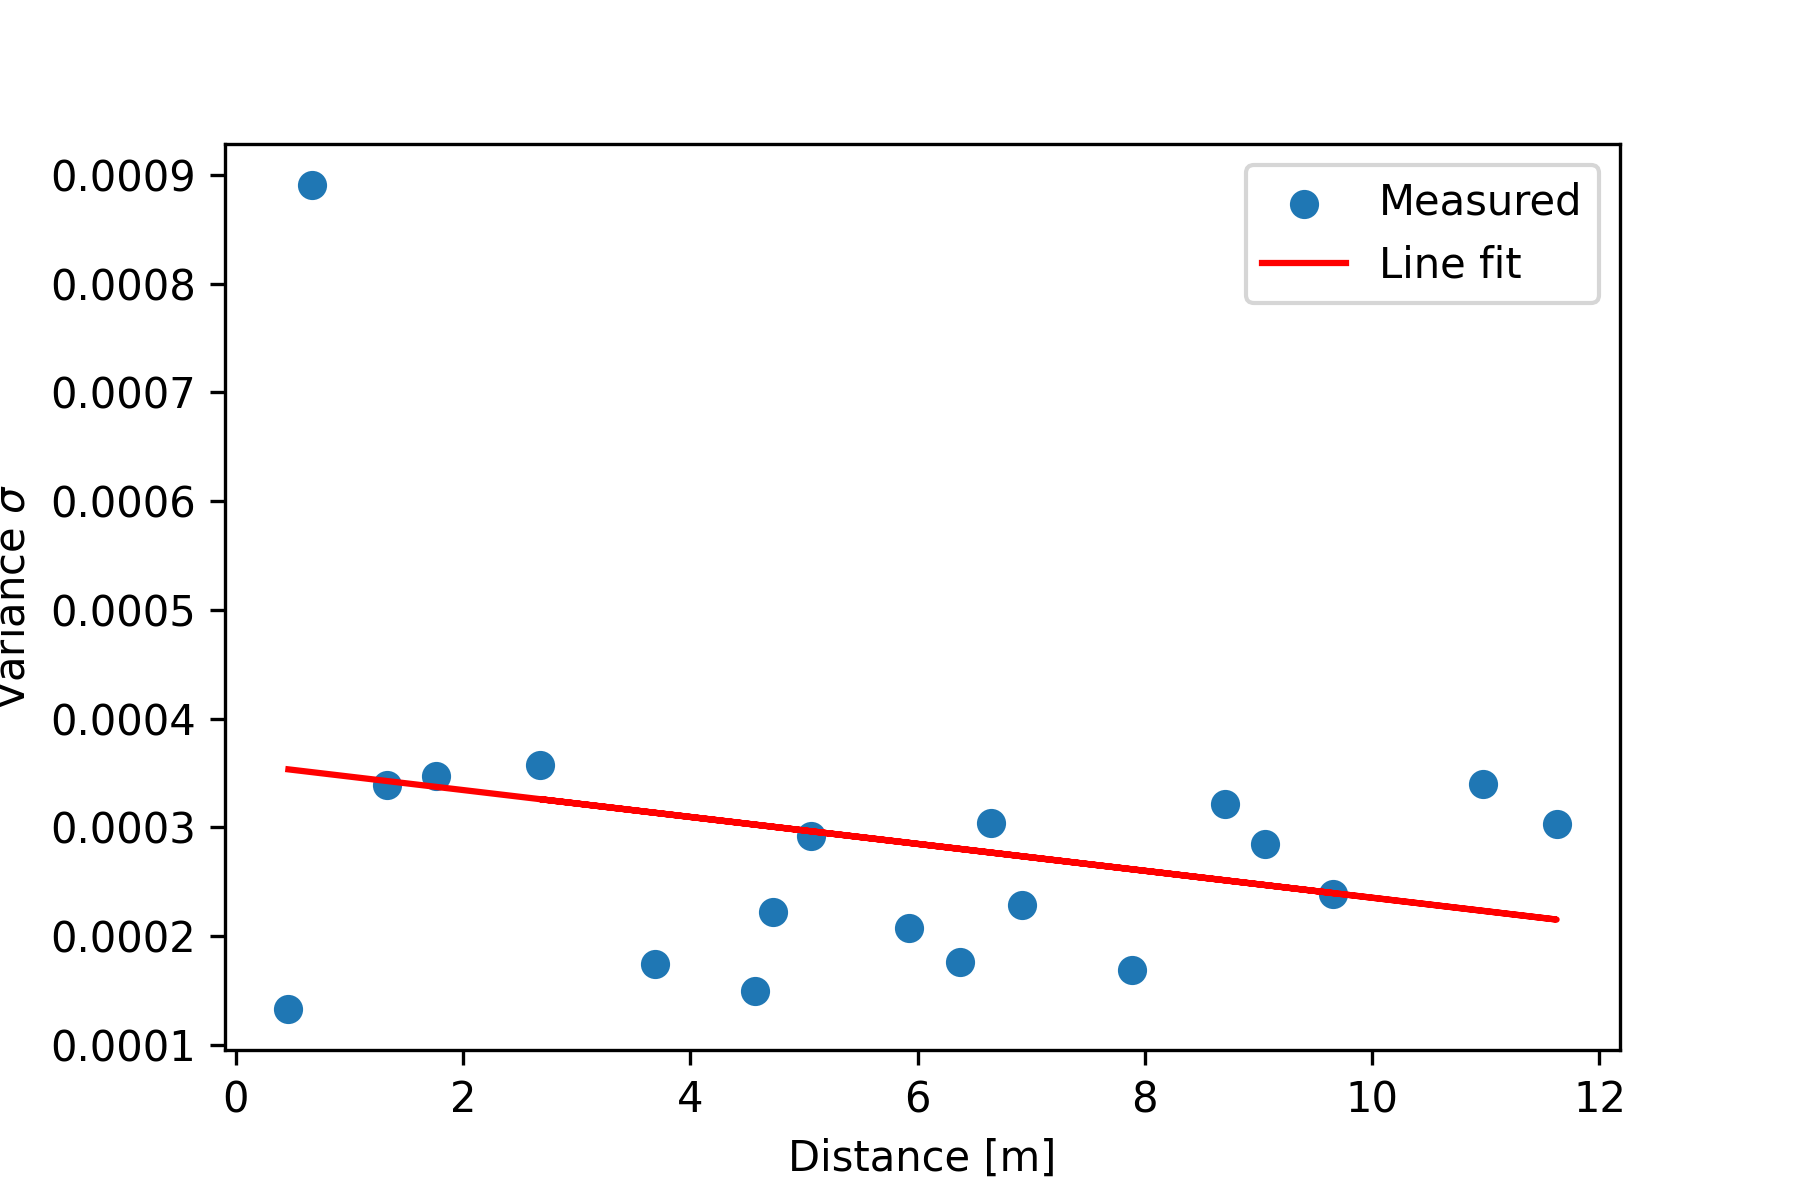
\includegraphics[width=\linewidth]{figures/dist_variance.png}
    \caption{Distance over measurement variance.}
    \label{fig:distance_var}
\end{figure}

% TODO: text
% TODO: what are these axis in 3D one  ? :) prob using the same figure as from the 2d plot
% TODO: look at the autocorr.py ??   

\begin{figure}[H]
    \centering
    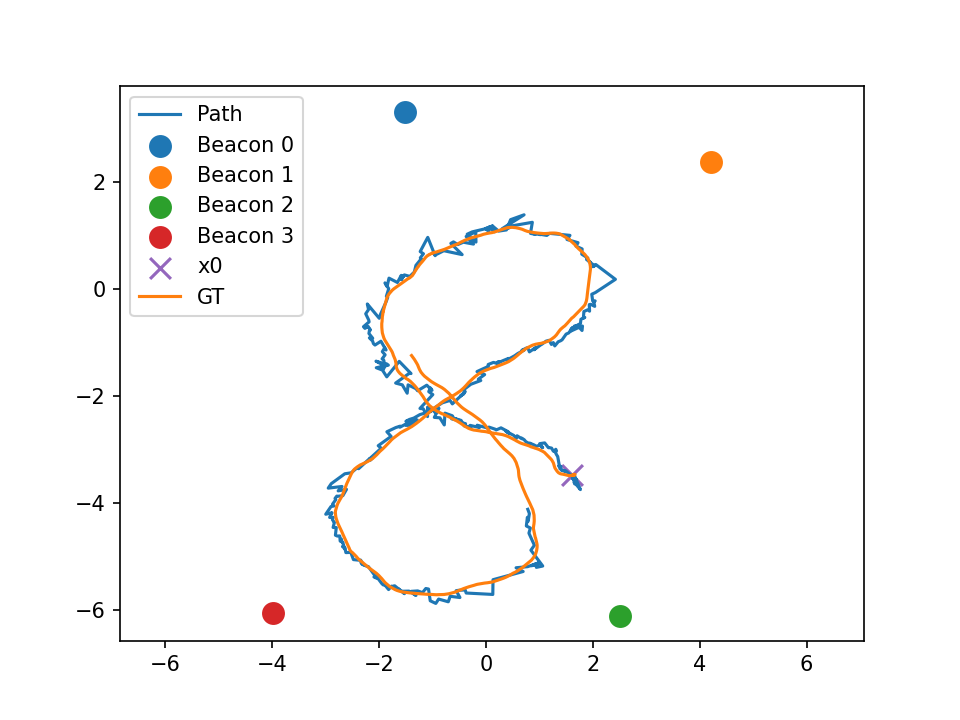
\includegraphics[width=\linewidth]{figures/2d_path.png}
    \caption{2D plot of experiment.}
    \label{fig:exp_2d_path}
\end{figure}
\begin{figure}[H]
    \centering
    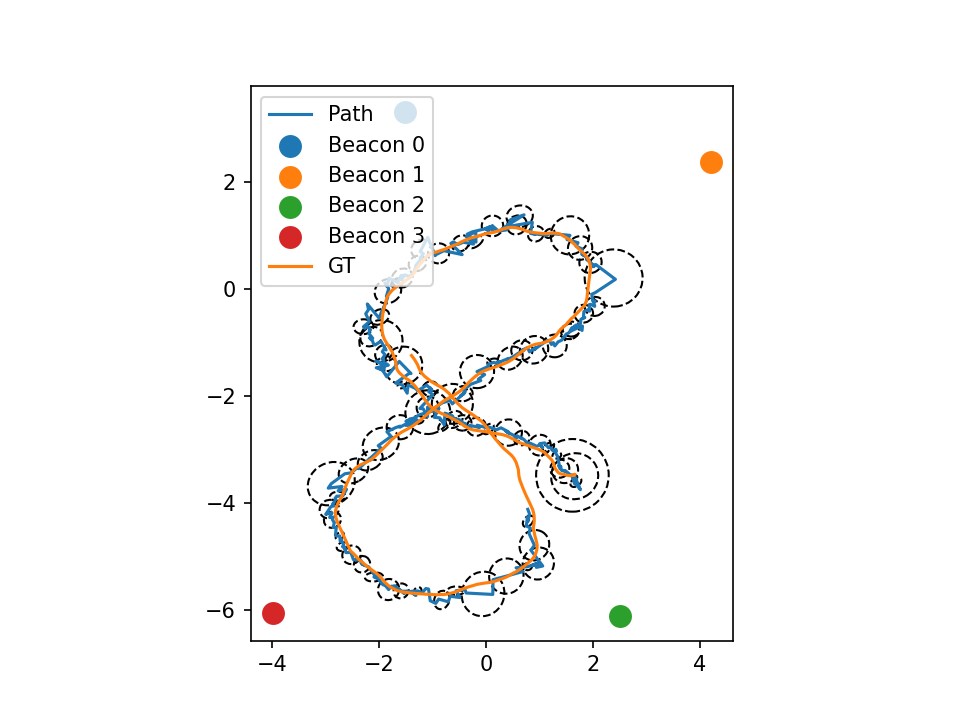
\includegraphics[width=\linewidth]{figures/2d_with_cov.png}
    \caption{2D plot of experiment with covariances.}
    \label{fig:exp_2d_path_covariances}
\end{figure}
\begin{figure}[H]
    \centering
    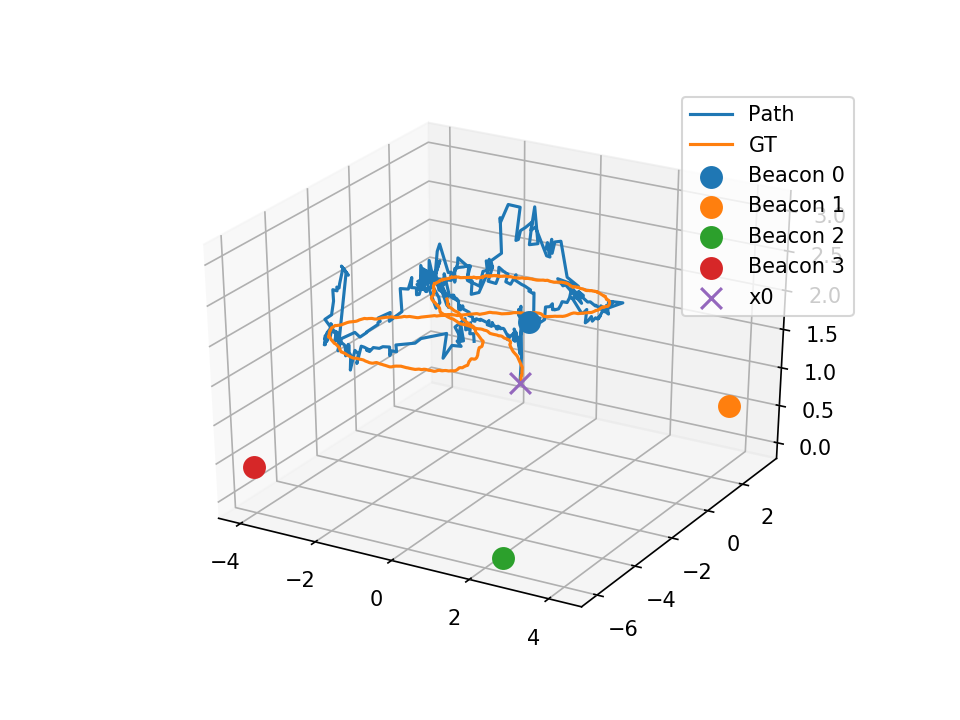
\includegraphics[width=\linewidth]{figures/3d_path.png}
    \caption{3D plot of experiment.}
    \label{fig:exp_3D_path}
\end{figure}

\label{EndOfText}

\newpage
\addcontentsline{toc}{section}{References}
\bibliography{document.bib}
\bibliographystyle{ieeetr}

\label{endOfDoc}
\end{document}
